\section{Model}

\subsection{Description}
\begin{figure}[h!]
    \centering
    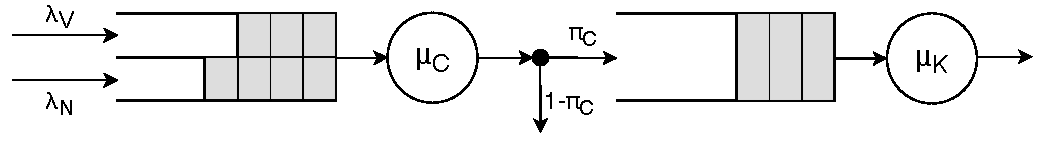
\includegraphics[width=\textwidth]{figs/qt_model.pdf}
    \caption{Schematic representation of the model of the bar.}
    \label{fig:model}
\end{figure}

In \cref{fig:model} you can see the model of the bar, where:
\begin{itemize}
    \item $\lambda_V$ is the average arrival rate for VIP customers;
    \item $\lambda_N$ is the average arrival rate for ``normal'' (i.e. non-VIP) customers;
    \item $\mu_C$ is the average service rate of the cashier ($r_{cashier}$);
    \item $\mu_K$ is the average service rate of the kitchen ($r_{kitchen}$);
    \item $\pi_C$ is the ratio of compound orders over the total, i.e. the 
        probability that an order is compound.
\end{itemize}

The cashier is modeled as a service center with two queues that are managed 
in an head-of-line-priority fashion.

The kitchen is modeled as a simple M/M/1 service center. Note that if VIP 
priority is introduced also in the kitchen, it will become identical to the 
cashier, mutatis mutandis.

\subsection{Assumptions}
The following assumptions were made when modeling the system:
\begin{itemize}
    \item No renegation: customers cannot leave the queue.
    \item No jockeying: VIP customers cannot move to the normal customers' queue.
    \item Infinite queueing space: there is no upper bound in the number of 
        customers in a queue.
    \item the interarrival times of VIP and normal customers are independent 
        RVs.
    \item the type of an order (simple or compound) is independent of the other
        orders.
    \item the service rate is the same for normal and VIP customers.
\end{itemize}

\subsection{Validation}
% TODO add something more or completely remove this section
The model exactly reflects the one dictated in the assignment.

\subsection{Stochastic model for the exponential scenario}
\begin{align}
    E[W^C_{V}] &= \frac{\lambda_V + \lambda_N}{(\mu_C-\lambda_{V})\mu_C} \\
    E[W^C_{N}] &= \frac{\lambda_V + \lambda_N}{(\mu_C-\lambda_{V}-\lambda_N)(\mu_C-\lambda_{V})} \\
    E[R^K] &= \frac{1}{\mu_K-p_C(\lambda_{V}+\lambda_{N})}
\end{align}